\chapter{Algorithms}
\label{chap:algorithms}
This chapter gives a description of the work-flow in problem generation and also detailed explanations of the algorithms used to generate problems for the tool. Primary problems along with hint questions are generated for the following broad domains:
\begin{itemize}
\item First and Follow
\item LL Parsing
\item SLR Parsing
\end{itemize}
The LL and SLR parsing problem domains have further sub-domains on which problems are generated by the tool. This chapter covers the algorithms for these sub-domains of problems, along with hint question generation algorithms and a few other auxiliary algorithms.
Problems in the LL Parsing domain involve the following categories:
\begin{itemize}
\item LL parsing table
\item LL parsing moves
\end{itemize}
Problems in the SLR Parsing domain involve the following categories:
\begin{itemize}
\item SLR canonical set
\item SLR parsing table
\item SLR parsing moves
\end{itemize}

The problem generation algorithms make a few assumptions on the grammar given as input. The following are the pre-conditions:
\begin{itemize}
\item Only Context Free Grammar (CFG) must be used.
\item If LL Parsing technique is to be used, then the grammar must not be left-recursive.
\item If the questions are to be generated for Parsing Moves of any Parsing Technique, then it is required that the grammar be unambiguous.
\end{itemize}

\section{Problem Generation Workflow}
\label{sec:Problem Generation}
This section describes the workflow of problem generation. Problems are generated for a specific domain which is chosen by the user. This information, along with the input grammar defines a set of possible problems which can be generated. These problems are known as primary problems. Each of these candidate problems are generated and given to the user to solve. Upon successfully solving one problem, the next candidate problem is presented to the user. The process of learning occurs when the user is not able to solve the presented primary problem. Hint questions are then generated to guide the user into reaching the correct solution and understanding her mistakes. The hint questions are of two types, based on the context on which they are generated:
\begin{itemize}
\item \textbf{H1:} This type of hint question is generated when an incorrect choice is marked by the user in her solution to the primary problem. The question tries to make the user realize that the choice marked is incorrect and should not be a part of the solution.
\item \textbf{H2:} This type of hint question is generated when a correct choice is omitted by the user in the solution set of choices. The generated question tries the help the user understand why the choice should be a part of the solution.
\end{itemize}

The workflow of problem generation is depicted below using several algorithms as depicted below. These algorithms depict the common structure of all algorithms across the various domains. However the exact algorithms for preprocessing, problem generation and hint generation are domain specific, and are elaborated in the subsequent sections.

\begin{algorithm}
\caption{Preprocess grammar to create required data structures}
\label{algo:preprocess}
\begin{algorithmic}[1]
\Function{preprocess}{$D$}
\State S := data structure on the basis of which questions will be generated.
\State A := auxiliary data structures required to compute S and display helpers to users.
\State \Return (S,A)
\EndFunction
\end{algorithmic}
\end{algorithm}

\begin{algorithm}
\caption{Generate questions for a specific domain}
\label{algo:generatequestions}
\begin{algorithmic}[1]
\Function{generate\textunderscore questions}{$D$}
\State (S,A) := \Call{preprocess}{$D$}
\ForAll{context in S}
\State P := \Call{generate\textunderscore primary\textunderscore question}{$context, D$}
\State $answered \gets false$
\While{$answered = false$}
\State $answered \gets \Call{evaluate\textunderscore primary\textunderscore question}{P, D}$
\EndWhile
\EndFor
\EndFunction
\end{algorithmic}
\end{algorithm}

\begin{algorithm}
\caption{Generate primary question based on a context in a specific domain}
\label{algo:generateprimary}
\begin{algorithmic}[1]
\Function{generate\textunderscore primary\textunderscore question}{$context, D$}
\State P := generated primary question based on D and context
\State \Return P
\EndFunction
\end{algorithmic}
\end{algorithm}

\begin{algorithm}
\caption{Evaluate primary question generated previously}
\label{algo:evaluateprimary}
\begin{algorithmic}[1]
\Require C = \{c | c $\in$ correct(P)\}
\Require I = \{c | c $\in$ incorrect(P)\}
\Function{evaluate\textunderscore primary}{$P, D$}
\State Display P to user
\State CHOICES := read set of choices from user
\If{$ CHOICES = C$}
\State Display "correct solution"
\State \Return true
\Else
\ForAll{choice in CHOICES}
\If{choice$\in$ I}
\State $H1 \gets \Call{generate\textunderscore hint\textunderscore question}{choice, P, D, 1}$
\State \Call{evaluate\textunderscore hint\textunderscore question}{$H1$}
\ElsIf{choice$\in$ C}
\State $C \gets C - \{choice\}$
\EndIf
\EndFor
\If{C$\neq \emptyset$}
\ForAll{choice $\in$ C}
\State $H2 \gets \Call{generate\textunderscore hint\textunderscore question}{choice, P, D, 2}$
\State \Call{evaluate\textunderscore hint\textunderscore question}{$H2$}
\State $H1 \gets \Call{generate\textunderscore hint\textunderscore question}{choice, P, D, 1}$
\State \Call{evaluate\textunderscore hint\textunderscore question}{$H1$}
\EndFor
\EndIf
\State \Return false
\EndIf
\EndFunction
\end{algorithmic}
\end{algorithm}

\begin{algorithm}
\caption{Generate hint question based on choice, problem and domain}
\label{algo:generatehint}
\begin{algorithmic}[1]
\Function{generate\textunderscore hint\textunderscore question}{$choice, P, D, type$}
\State H := generated hint question based on type, options of P, choice and domain D
\State \Return H
\EndFunction
\end{algorithmic}
\end{algorithm}

\begin{algorithm}
\caption{Evaluate hint question generated previously}
\label{algo:evaluatehint}
\begin{algorithmic}[1]
\Require C := correct choice for H
\Function{evaluate\textunderscore hint\textunderscore question}{$H$}
\State $correct \gets false$
\While{$\neg correct$}
\State display H
\State read choice
\If{choice = C}
\State correct = true
\Else
\State correct = false
\EndIf
\EndWhile
\State display "correct solution"
\EndFunction
\end{algorithmic}
\end{algorithm}

\section{First and Follow}
\label{sec:firstandfollow}
This domain of the problems attempts to teach First and Follow sets in compilers. The procedures that are specific to this domain include preprocessing, primary problem generation and hint question generation. We shall describe each of these procedures below.

\subsection{First}
\label{subsec:ff-first}

Preprocessing for generation of questions in the First domain involves computation of first sets for all non-terminals in the grammar. This is depicted in algorithm \ref{algo:preprocess-first}. Algorithm \ref{algo:primary-first} shows how primary problems are generated for a specific context derived from the preprocessing stage. Further, algorithm \ref{algo:hint-first} explains the procedure for generating hint questions of a specified type and based on a choice from the solution set.

\begin{algorithm}
\caption{Preprocessing for First}
\label{algo:preprocess-first}
\begin{algorithmic}[1]
\Function{preprocess\textunderscore first}{$G$}
\State N := set of all non-terminals in grammar G
\State S := table for storing all first sets
\ForAll{n in N}
\State F := \{ t | t$\in$ first(n)\}
\State S[n] = F
\EndFor
\State \Return S
\EndFunction
\end{algorithmic}
\end{algorithm}

\begin{algorithm}
\caption{Primary problem generation for First}
\label{algo:primary-first}
\begin{algorithmic}[1]
\Function{generate\textunderscore primary\textunderscore question\textunderscore first}{$context, S$}
\State Q := "Which symbols should be included in FIRST[context] ?"
\State F = S[context]
\State \Return (Q, F)
\EndFunction
\end{algorithmic}
\end{algorithm}

In algorithm \ref{algo:hint-first}, hint question H (H1) contains all the rules described in \ref{ssubsec:preliminary}, required to generate first set for each symbol in the grammar. Answer to this hint question contains the rule number which is satisfied by the choice.
\begin{algorithm}
\caption{Hint question generation for First}
\label{algo:hint-first}
\begin{algorithmic}[1]
\Function{generate\textunderscore hint\textunderscore question\textunderscore first}{$choice, P, D, type, context$}
\If{type = 1}
\State H := "According to which of the rules of first, choice is a part of FIRST[context] ? 1. If X is a terminal, ..... 4. No valid rule for this symbol."
\If{choice$\in$ I}
\State A := 4
\ElsIf{choice$\in$ C}
\State A := 1 or 2 or 3
\EndIf
\ElsIf{type = 2}
\State H := "Should choice be included in FIRST[context] ?"
\State A := "Yes"
\EndIf
\State \Return (H, A)
\EndFunction
\end{algorithmic}
\end{algorithm}

\subsection{Follow}
\label{subsec:ff-follow}

Preprocessing for generation of problems in the Follow domain, involves computing First and Follow sets for the given grammar. This is shown in algorithm \ref{algo:preprocess-follow}. The procedures for primary problem generation and hint question generation are shown in algorithms \ref{algo:primary-follow} and \ref{algo:hint-follow} respectively.

\begin{algorithm}
\caption{Preprocessing for Follow}
\label{algo:preprocess-follow}
\begin{algorithmic}[1]
\Function{preprocess\textunderscore follow}{$G$}
\State N := set of all non-terminals in grammar G
\State S := table for storing all follow sets
\ForAll{n in N}
\State F := \{ t | t$\in$ follow(n)\}
\State S[n] = F
\EndFor
\State \Return S
\EndFunction
\end{algorithmic}
\end{algorithm}

\begin{algorithm}
\caption{Primary question generation for Follow}
\label{algo:primary-follow}
\begin{algorithmic}[1]
\Function{generate\textunderscore primary\textunderscore question\textunderscore follow}{$context$}
\State Q := "Which symbols should be included in FOLLOW[context] ?"
\State F = S[context]
\State \Return (Q, F)
\EndFunction
\end{algorithmic}
\end{algorithm}

In algorithm \ref{algo:hint-follow}, hint question H (H1) contains all the rules described in \ref{ssubsec:preliminary}, required to generate follow set for each symbol in the grammar. Answer to this hint question contains the rule number which is satisfied by the choice.

\begin{algorithm}
\caption{Hint question generation for Follow}
\label{algo:hint-follow}
\begin{algorithmic}[1]
\Function{generate\textunderscore hint\textunderscore question\textunderscore follow}{$choice, type, context$}
\If{type = 1}
\State H := "According to which of the rules of follow, choice is a part of FOLLOW[context] ? 1. \$ is in FOLLOW(S), ..... 4. No valid rule for this symbol."
\If{choice$\in$ I}
\State A := 4
\ElsIf{choice$\in$ C}
\State A := 1 or 2 or 3
\EndIf
\ElsIf{type = 2}
\State H := "Should choice be included in FOLLOW[context] ?"
\State A := "Yes"
\EndIf
\State \Return (H, A)
\EndFunction
\end{algorithmic}
\end{algorithm}

\section{LL Parsing}
\label{llparsing}

This domain of problems attempts to teach users the LL parsing technique in compilers. Similar to the First and Follow domain, the same procedures have different algorithms that are specific to this domain. We shall be describing these procedures below. This domain is further divided into two sub-domains: LL parsing table and LL parsing moves. The following subsections cover these sub-domains. 

\subsection{LL Parsing Table}
\label{subsec:lltable}

This sub-domain of problems attempts to teach users how to build a LL parsing table. Problems in this sub-domain involve filling out entries in the cells of a LL parsing table. The problems in this sub-domain are split into two levels, depending on the approach used for learning. These levels differ in the type of hint questions that are generated. Both these levels involve generation of a primary question, which instructs the user to fill up missing cells in the parsing table. It is when the user makes a wrong attempt, that the levels come into play:
\begin{itemize}
\item \textbf{Level 1:} The hint questions involve generation of a question of type H1, if an incorrect entry is made in one of the cells. If a correct entry is omitted in the cell, a question of type H2 is generated. This is similar to the work-flow of problem generation in the First and Follow domain. 
\item \textbf{Level 2:} In this level, only one category of hint is generated. It is assumed here that the grammar is unambiguous and hence a cell cannot contain more than one entry. Thus, for each incorrect cell entry in the table, a corresponding input string is generated. This is the shortest possible input string for that cell entry. Using the entries filled up by the user in the parsing table, a sequence of parsing moves on the generated input string is displayed to the user as the hint. The user is then asked to correct the erroneous cell entry in the parsing table, using this information.
\end{itemize}

The preprocessing required for question generation on LL parsing table is shown in algorithm \ref{algo:preprocessing-lltable}. Primary problem generation is described using algorithm \ref{algo:primary-lltable}. Hint question for level 1 is depicted in algorithm \ref{algo:hint-lltable}. Input string generation is described in section \ref{ssec:inputgen}.

Instead of filling all the entries of LL parsing table, the user is asked to fill some entries of the table. For this purpose, Algorithm \ref{algo:preprocessing-lltable} uses 4 random numbers. These random numbers are generated on the index of cells of LL parsing table. The algorithm picks those random indexes one by one and generates primary question along with hint questions.

\begin{algorithm}
\caption{Preprocessing for LL parsing table}
\label{algo:preprocessing-lltable}
\begin{algorithmic}[1]
\Function{preprocessing\textunderscore lltable}{$G, First, Follow, T$}
\State N := set of all non-terminals in grammar G
\State L := LL parsing table 
\ForAll{n in N}
\State D := table containing all the cells of the corresponding n
\ForAll{t in T}
\State F := \{ x | x$\in$ cell[n][t]\}
\State D[t] = F
\EndFor
\State L[n] = D
\EndFor
\State R := set containing 4 random numbers on indexes of LL table
\State S = \{\} \Comment set containing cells to be questioned
\ForAll{r in R}
\State index := choose random cell index in L
\State E := context corresponding to index
\State S = S $\cup$ E
\EndFor
\State \Return (L, S)
\EndFunction
\end{algorithmic}
\end{algorithm}

\begin{algorithm}
\caption{Primary problem generation for LL parsing table}
\label{algo:primary-lltable}
\begin{algorithmic}[1]
\Function{generate\textunderscore primary\textunderscore question\textunderscore lltable}{$context$}
\State Q := "Which grammar rules should be included in the context cell of the LL parsing table ?"
\State index := choose random cell index in table
\State n := row name of cell referenced by index
\State t := column name of cell referenced by index
\State F = L[n][t]
\State \Return (Q, F)
\EndFunction
\end{algorithmic}
\end{algorithm}

\begin{algorithm}
\caption{Hint question generation for LL parsing table}
\label{algo:hint-lltable}
\begin{algorithmic}[1]
\Function{generate\textunderscore hint\textunderscore question\textunderscore lltable}{$choice, type$}
\If{type = 1}
\State H := "According to which of the rules of ll parsing table, choice belongs to the context cell ? 1. 1. If A $\rightarrow$ $\alpha$ is a production ..... 4. No valid rule."
\If{choice$\in$ I}
\State A := 4
\ElsIf{choice$\in$ C}
\State A := 1 or 2 or 3
\EndIf
\ElsIf{type = 2}
\State H := "Should choice be a part of the context cell ?"
\State A := "Yes"
\EndIf
\State \Return (H, A)
\EndFunction
\end{algorithmic}
\end{algorithm}

\subsubsection{Input String Generation}
\label{ssec:inputgen}

This section describes the procedure for input string generation for problems in the LL parsing domain. Algorithms \ref{algo:inputstr gen} through \ref{algo:graph gen} show this procedure.

The following example (\ref{ex:inputstr}) depicts the working of the procedure:
\begin{example}
\label{ex:inputstr}
Suppose the grammar is \\
E $\to$ T E' \\
E' $\to$ + T E' | $\epsilon$ \\
T $\to$ F T' \\
T' $\to$ * F T' | $\epsilon$ \\
F $\to$ ( E ) | id

The graph generated by the algorithm for this grammar is shown in Figure \ref{fig:Grammar Graph}.
\begin{figure}
\centering
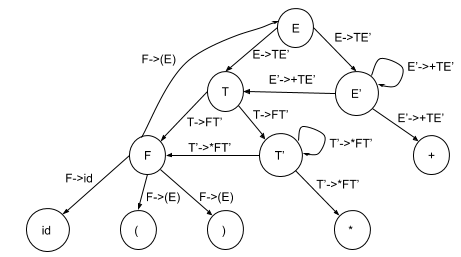
\includegraphics[width=0.8\textwidth]{GrammarGraph.png}
\caption{Graph generated on applying algorithm \ref{algo:graph gen}}
\label{fig:Grammar Graph}
\end{figure}

The node containing the start symbol becomes the source node. Then, we apply Dijkstra's Algorithm to find shortest path from the source to every other node in the graph. The resultant tree is shown in Figure \ref{fig:Dijkstra Tree 1}.
\begin{figure}
\centering
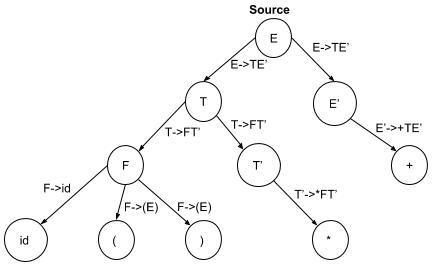
\includegraphics[width=0.8\textwidth]{DijkstraTree1.png}
\caption{Tree after applying Dijkstra Algorithm first time}
\label{fig:Dijkstra Tree 1}
\end{figure}

If the user made an incorrect entry in M[T'][)] of LL Parsing Table (where M refers to the data structure containing the parsing table), then the node corresponding to T' becomes the destination node. The next step in the algorithm is to find the shortest path from the source to the destination in the tree using Dijkstra Algorithm. The path in the tree is shown in Figure \ref{fig:Path 1}.

\begin{figure}
\centering
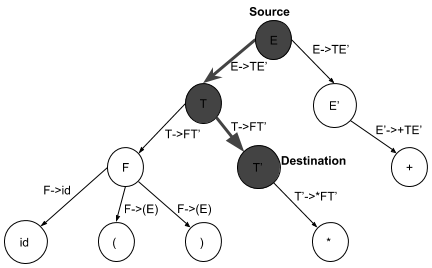
\includegraphics[width=0.8\textwidth]{Path1.png}
\caption{Path in the tree from E to T'}
\label{fig:Path 1}
\end{figure}

Now, in order to build the input string, we have used a stack containing the symbols in the grammar. The stack is just like the stack used for LL Parsing Moves. It consists of all the symbols that occur in the path of input string generation. The stack consists of '\$' initially. All the keys corresponding to the nodes and the symbols on the edges, obtained in the path from source to destination, are pushed on to the stack in the order in which the path is accessed.

If a non-terminal appears on the top of the stack then,
\begin{itemize}
\item if it is the key of a node in the path, the outgoing edge from this node in the path, is pushed on to the stack in reverse order.
\item otherwise the minimum length rule in the grammar for this non-terminal, is pushed on to the stack in reverse order.
\end{itemize}
If a terminal symbol appears on top of the stack, it is popped from the stack and appended to the input string.

Following is the configuration obtained by using the path from E to T' shown in Figure \ref{fig:Path 1}.
\begin{center}
\begin{tabular}{ |c|c| } 
 \hline
 \textbf{stack} & \textbf{input string} \\
 \hline
 \$E & \\
 \$E'T & \\
 \$E'T'F & \\
 \hline
\end{tabular}
\end{center}

On top of the stack, we have symbol F, which is not in the path from E to T', so we replace it by the shortest rule in the grammar for this non-terminal (F $\to$ id). The configuration now becomes
\begin{center}
\begin{tabular}{ |c|c| } 
 \hline
 \textbf{stack} & \textbf{input string} \\
 \hline
 \$E'T'id & \\
 \hline
\end{tabular}
\end{center}

Now, as a terminal appears on top of the stack, it is popped from the stack and becomes a part of the input string. Now the configuration becomes
\begin{center}
\begin{tabular}{ |c|c| } 
 \hline
 \textbf{stack} & \textbf{input string} \\
 \hline
 \$E'T' & id \\
 \hline
\end{tabular}
\end{center}

Now, we have T'(destination) on top of the stack. As there is no rule of T' in the grammar which contains ), we have to find a path from T' to ). For this purpose T' now becomes the source node. Again Dijkstra's algorithm is applied, to find shortest paths from the new source to all other nodes in the graph. Figure \ref{fig:Dijkstra Tree 2} shows the tree obtained after applying Dijkstra algorithm.
\begin{figure}
\centering
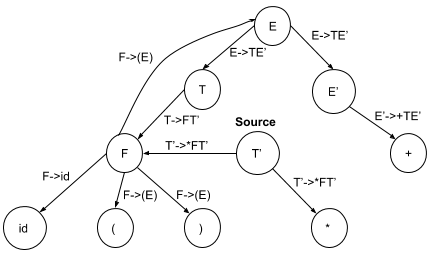
\includegraphics[width=0.8\textwidth]{DijkstraTree2.png}
\caption{Tree after applying Dijkstra Algorithm second time}
\label{fig:Dijkstra Tree 2}
\end{figure}

Now, the node corresponding to ) becomes the destination node. The path from T' to ) is picked up from this tree and is shown in Figure \ref{fig:Path 2}.
\begin{figure}
\centering
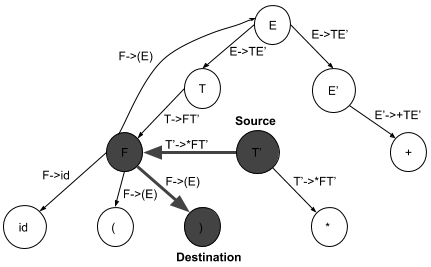
\includegraphics[width=0.8\textwidth]{Path2.png}
\caption{Path in the tree from T' to )}
\label{fig:Path 2}
\end{figure}

As T' is on top of the stack, it is popped from the stack and the outgoing edge from T' on the path is pushed on to the stack in reverse order. Same procedure, as described above, is applied on further steps.
\begin{center}
\begin{tabular}{ |c|c| } 
 \hline
 \textbf{stack} & \textbf{input string} \\
 \hline
 \$E'T'F* & id \\
 \$E'T'F & id * \\
 \$E'T')E( & id * \\
 \$E'T')E &	id * ( \\
 \$E'T')E'T & id * ( \\
 \$E'T')E'T'F &	id * ( \\
 \$E'T')E'T'id & id * ( \\
 \$E'T')E'T' & id * ( id \\
 \$E'T')E'$\epsilon$ & id * ( id \\
 \$E'T')E' & id * ( id \\
 \$E'T')$\epsilon$ & id * ( id \\
 \$E'T') & id * ( id \\
 \$E'T' & id * ( id ) \\
 \$E'$\epsilon$ & id * ( id ) \\
 \$E' & id * ( id ) \\
 \$$\epsilon$ & id * ( id ) \\
 \$ & id * ( id ) \\
 \hline
\end{tabular}
\end{center}

Now we have reached the end of the stack and obtained the input string for the cell M[T][)] filled incorrectly by the user. This input string is then used to generate hint questions.

\end{example}

% input string generation
\begin{algorithm}
\caption{Input string generation for LL parsing table}
\label{algo:inputstr gen}
\begin{algorithmic}[1]
\Function{generate\textunderscore input\textunderscore string}{$G, N, t$}
\State (E,V,LABELS) = \Call{generate\textunderscore graph}{$G$}
\State MINRULES = \Call{minrules\textunderscore gen}{$G$}
\State S := start symbol for G
\State SHORTEST = \Call{djikstra}{$E,V,S$}
\State PATH = SHORTEST[N] \Comment shortest path from S to N
\State STACK = \{\$S\}
\State PARTIAL = ""
\State (STACK,PARTIAL) = \Call{find\textunderscore input}{$PARTIAL, PATH, LABELS, MINRULES, G, STACK$}
\State SH = \Call{djikstra}{$E,V,N$}
\State PH = SH[t] \Comment shortest path from N to t
\State (STACK,PARTIAL) = \Call{find\textunderscore input}{$PARTIAL, PH, LABELS, MINRULES, G, STACK$}
\State INPUTSTRING = \Call{empty\textunderscore stack}{$G, STACK, PARTIAL, MINRULES$}
\State \Return INPUTSTRING
\EndFunction
\end{algorithmic}
\end{algorithm}

\begin{algorithm}
\caption{Generate partial input string}
\label{algo:find input}
\begin{algorithmic}[1]
\Function{find\textunderscore input}{$PARTIAL, PATH, LABELS, MINRULES, G, STACK$}
\State NT := set of all non-terminals in G
\While{PATH !empty}	
\State next = \Call{next}{$PATH$}
\State top = \Call{pop}{$STACK$}
\If{top = next}
\State dest = \Call{successor}{$PATH, next$}
\State label = \Call{reverse}{$LABELS[(next,dest)]$}
\State \Call{push}{$STACK, label$}
\Else
\If{top\in NT}
\State minr = \Call{reverse}{$MINRULES[top]$} \Comment reverses the minimum length rule for top
\State \Call{push}{$STACK, minr$}
\Else
\State PARTIAL = \Call{append}{$PARTIAL, top$} 
\EndIf
\EndIf
\EndWhile
\State \Return (STACK, PARTIAL)
\EndFunction
\end{algorithmic}
\end{algorithm}

\begin{algorithm}
\caption{Empty stack and generate final input string}
\label{algo:stack empty}
\begin{algorithmic}[1]
\Function{empty\textunderscore stack}{$G, STACK, PARTIAL, MINRULES$}
\State NT := set of all non-terminals in G
\While{\Call{top}{$STACK$}\neq \$}
\State top = \Call{pop}{$STACK$}
\If{top\in NT}
\State minr = \Call{reverse}{$MINRULES[top]$} \Comment reverses the minimum length rule for top
\State \Call{push}{$STACK, minr$}
\Else
\State PARTIAL = \Call{append}{$PARTIAL, top$} 
\EndIf				
\EndWhile
\State \Return PARTIAL
\EndFunction
\end{algorithmic}
\end{algorithm}

\begin{algorithm}
\caption{Generate minimum length rules for each non-terminal in grammar}
\label{algo:minrule gen}
\begin{algorithmic}[1]
\Function{minrules\textunderscore gen}{$G$}
\State RULES := table containing rules for every non-terminal in G
\State N := set of all non-terminals in G
\State MINRULES := table containing all minimum length rules of every n\in N
\ForAll{n in N}
\State R = RULES[n] \Comment set containing all rules of n
\State Rm = \Call{min}{$R$}
\State MINRULES[n] = Rm
\EndFor
\State \Return MINRULES
\EndFunction
\end{algorithmic}
\end{algorithm}

\begin{algorithm}
\caption{Graph generation from grammar}
\label{algo:graph gen}
\begin{algorithmic}[1]
\Function{generate\textunderscore graph}{$G$}
\State RULES := table containing rules for every non-terminal in G
\State N := set of non-terminals in G
\State T := set of terminals in G
\State V = N\cup T \Comment set of vertices in graph
\State E = \{\} \Comment set of edges in graph
\State LABELS := table with keys belonging to E
\ForAll{n in N}
\State R = RULES[n]
\State DEST = \{\}
\ForAll{rule in R}
\ForAll{symbol in rule}
\State DEST = DEST\cup \{symbol\}
\State E = E\cup (n,symbol)
\If{$LABELS[(n,symbol)] = null \parallel \Call{length}{rule} < \Call{length}{LABELS[(n,symbol)]}$}
\State LABELS[(n,symbol)] = rule
\EndIf
\EndFor
\EndFor
\EndFor
\State \Return (E,V, LABELS)
\EndFunction
\end{algorithmic}
\end{algorithm}

% end input string generation

\subsection{LL Parsing Moves}
\label{subsec:llmoves}

This sub-domain of problems attempts to teach users how to parse an input string using the LL parsing table for the corresponding grammar. The problems in this sub-domain involve predicting the next move in a sequence of parsing moves. The algorithms specific to this domain of problems include preprocessing, primary problem generation and hint question generation. The procedure for preprocessing is shown in algorithm \ref{algo:preprocessing-llmoves}. Primary problem generation involves questions that are of the MCSA type. This is shown in algorithm \ref{algo:primary-llmoves}. Hint questions H1 and H2 are generated using the procedure described in algorithm \ref{algo:hint-llmoves}.

\begin{algorithm}
\caption{Preprocessing for LL parsing moves}
\label{algo:preprocessing-llmoves}
\begin{algorithmic}[1]
\Function{preprocess\textunderscore llmoves}{$G, L, s$}
\State I := Valid input string for parsing with \$ at the end
\State M := sequence of moves of parsing on input string
\State STACK := stack containing \$ and s, with s on top
\State index = 0    \Comment move number
\While{\Call{top}{STACK}\neq \$}
\State move = llmove[I]
\State M[index] = move
\State index = index + 1
\EndWhile
\State r := random number on index of moves
% \State move = M[r]
% \State S := data structure for moves
% \State S[0] = M[r]
% \State index = 1    \Comment move number
% \While{M !empty}
% \State S[index] = M[r+index]
% \EndWhile
\State \Return (M, r)
\EndFunction
\end{algorithmic}
\end{algorithm}

\begin{algorithm}
\caption{Primary problem generation for LL parsing moves}
\label{algo:primary-llmoves}
\begin{algorithmic}[1]
\Function{generate\textunderscore primary\textunderscore question\textunderscore llmoves}{$context$}
\State S := sequence of moves from index 0 to r-1   \Comment r is move number
\State Q := S, "What will be the next move?"
\State F = M[r]
\State \Return (Q, F)
\EndFunction
\end{algorithmic}
\end{algorithm}

\begin{algorithm}
\caption{Hint question generation for LL parsing moves}
\label{algo:hint-llmoves}
\begin{algorithmic}[1]
\Function{generate\textunderscore hint\textunderscore question\textunderscore llmoves}{$choice, type$}
\If{type = 1}
\State H := "By which of the following rule, do you think choice should be the next move? 1. If X = a = \$, ..... 4. No valid rule."
\If{choice$\in$ I}
\State A := 4
\ElsIf{choice$\in$ C}
\State A := 1 or 2 or 3
\EndIf
\ElsIf{type = 2}
\State H := "Probably context should be the next move. What do you think ?"
\State A := "Yes"
\EndIf
\State \Return (H, A)
\EndFunction
\end{algorithmic}
\end{algorithm}

\section{SLR Parsing}
\label{slrparsing}

This domain of problems attempts to teach the SLR parsing technique to users. The types of questions covered in this domain include filling up entries in certain data structures. This domain is further divided into sub-domains: SLR canonical set, SLR parsing table and SLR parsing moves. These are described in the subsections that follow. 

\subsection{SLR Canonical Set}
\label{subsec:slrcanonical}

SLR canonical sets have been described in section \ref{para:Canonical Set} of chapter \ref{chap:background}. Questions are generated on concepts involving item sets (described in \ref{para:Canonical Set}). These questions involve filling up entries in these  item sets and choosing correct item sets for a particular context. These questions are divided into two categories - SLR closure and SLR goto.

\subsubsection{SLR Closure}
\label{ssec:slrclosure}
SLR Closure of an item set have been described in section \ref{para:Canonical Set} of chapter \ref{chap:background}. In short it is a function which is used to build a SLR canonical set. The problems generated in this sub-domain attempt to teach users to combine SLR items into different item sets. The problems involve completion of the incomplete item sets. A incomplete item set is the result of applying GOTO function on a complete item set.

The algorithms specific to this sub-domain are preprocessing, primary problem generation and hint question generation. The procedure for preprocessing is shown in algorithm \ref{algo:preprocessing-slrclosure}, for primary problem generation in algorithm \ref{algo:primary-SlrClosure} and for hint generation in algorithm \ref{algo:hint-slrclosure}.

\begin{algorithm}
\caption{Preprocessing for SLR Closure}
\label{algo:preprocessing-slrclosure}
\begin{algorithmic}[1]
\Function{preprocess\textunderscore slrclosure}{$G, s$}
\State aug := \{$s'\rightarrow s$\} \Comment s' is the new start symbol
\State aug = aug\cup G
\State C = \Call{SLRCanonicalSet}{aug}  \Comment SLR canonical set
\State R := set containing 4 random numbers on indexes of C
\State S = \{\} \Comment set containing item sets to be questioned
\ForAll{r in R}
\State index := choose random item set index in C
\State E := context corresponding to index
\State S = S $\cup$ E
\EndFor
\State \Return S
\EndFunction
\end{algorithmic}
\end{algorithm}

\begin{algorithm}
\caption{Primary problem generation for SLR Closure}
\label{algo:primary-SlrClosure}
\begin{algorithmic}[1]
\Function{generate\textunderscore primary\textunderscore question\textunderscore SLRClosure}{$context$}
\State Q := "If I is the set of items context, then which items will be contained in CLOSURE(I) ?"
\State itemset = C[context] \Comment item set corresponding to closure of context
\State \Return (Q, itemset)
\EndFunction
\end{algorithmic}
\end{algorithm}

\begin{algorithm}
\caption{Hint question generation for SLR Closure}
\label{algo:hint-slrclosure}
\begin{algorithmic}[1]
\Function{generate\textunderscore hint\textunderscore question\textunderscore slrclosure}{$choice, type$}
\If{type = 1}
\State H := "By which of the following rule, do you think choice should be contained in CLOSURE(context) ? 1. Every item in I is in CLOSURE(I) ...... 3. No valid rule."
\If{choice$\in$ I}
\State A := 3
\ElsIf{choice$\in$ C}
\State A := 1 or 2
\EndIf
\ElsIf{type = 2}
\State H := "Should choice be contained in CLOSURE(I) ?"
\State A := "Yes"
\EndIf
\State \Return (H, A)
\EndFunction
\end{algorithmic}
\end{algorithm}

\subsubsection{SLR GOTO}
\label{ssec:slrgoto}

The two types of questions generated are distinguished on the basis of levels. They are described below:
\begin{itemize}
\item \textbf{Level 1:}
\item \textbf{Level 2:}
\end{itemize}

\subsection{SLR Parsing Table}
\label{subsec:slrtable}

\subsection{SLR Parsing Moves}
\label{subsec:slrmoves}

\begin{algorithm}
\caption{}
\label{algo:}
\begin{algorithmic}[1]
\Function{}{}
\EndFunction
\end{algorithmic}
\end{algorithm}

We have used three types of questions as described in chapter \ref{chap:overview}, out of which, Question 1 is the primary question and Questions 2 and 3 are hint questions of type 1 (H1) and 2 (H2) respectively. These questions are used for all the parsing techniques. However in some techniques, different types of questions are added by creating levels in them.

As an example, consider the LL parsing technique. In the LL Parsing table, we have created two levels: Level 1 uses the same flow as described, but level 2 uses the input strings generated by the tool for wrongly entered cells (in the hint questions). Primary questions remain the same for both levels. The algorithm for level 2 is described in section %\ref{sec:LL Table Level 2}.

Similarly for the GOTO function of SLR Canonical set, we have created two levels: Level 1 uses the same algorithm described below. However for level 2, there is a change in the type of questions generated and hence the algorithm is different. The algorithm for level 2 of GOTO is described in section \ref{sec:Goto Level 2}.

\begin{algorithm}                     
\begin{algorithmic} [1]
\If{stack is not empty}, 
\State Take one value out of the stack.
\If{state is 1}
\If{answer is not null}
\State Separate the incorrect options from the answer.
\State Also find the correct options which are not marked as the answer.
\If{there are no incorrect options and left out correct options}
\State assign answer = null and go to step 4.
\Else
\State Assign state = 2 and answer = null.
\EndIf
\Else
\State Display Question 1 and collect the marked options as answer.
\EndIf
\EndIf
\If{state is 2}
\If{answer is null or answer is right}
\If{there are incorrect options}
\State Pick one incorrect option
\State Display and take answer of Question 2 for this incorrect option.
\Else
\State Assign state = 4 and answer = null.
\EndIf
\Else
\State Display and take answer of Question 2 for the current incorrect option.
\EndIf
\EndIf
\If{state is 4}
\If{answer is null or answer is right}
\If{there are correct options which were left out in the answer}
\State Take one correct option and assign state = 3.
\Else
\State Assign state = 1, answer = null
\State Display Question 1 and collect the marked options as answer.
\EndIf
\Else
\State Display and take answer of Question 2 for the current incorrect option.
\EndIf
\EndIf
\If{state is 3}
\If{answer is right}
\State Assign state = 4
\State Display and take answer of Question 2 for the current correct option.
\Else
\State Display and take answer of Question 3 for the current correct option.
\EndIf
\EndIf
\EndIf
\end{algorithmic}
\end{algorithm}

\section{Level 2 of GOTO in SLR Canonical Set}
\label{sec:Goto Level 2}
In SLR Canonical set, choice for CLOSURE and GOTO function is given to generate questions on them. Different kinds of question are added for GOTO function by creating another level in it.

In this level of GOTO, we have again used three types of questions. But the content of the questions is different here. Question 1, which is the main question, contains the reverse question of the one in level 1 of GOTO. Question 2 and 3 are the hint questions but with different content.
\begin{example}
For the grammar used in \ref{ex:First}, questions are of the form:
\begin{itemize}
\item \textbf{Question 1 (Main Question):} In GOTO(I, X), if X is the grammar symbol E, then which of the following itemsets can act as I to get itemset {[E' $\to$ +E.]} as result ?

\textbf{Options:}

I0: T $\to$ .1 \quad E'' $\to$ .E \quad T $\to$ .0 \quad E $\to$ .TE'

I1: E $\to$ T.E' \quad E' $\to$ . \quad E' -> .+E

I2: T $\to$ 1.

I3: T $\to$ 0.

I4: E'' $\to$ E.

I5: T $\to$ .0 \quad E $\to$ .TE' \quad E' $\to$ +.E \quad T $\to$ .1

I6: E $\to$ TE'.    

I7: E' $\to$ +E.

\item \textbf{Question 2 (Hint Question, type 1):} Should GOTO(I, X), where I is the itemset containing {[T $\to$ .0], [T $\to$ .1], [E $\to$ .TE'], [E'' $\to$ .E]} and X is the symbol E, result in the itemset {[E' $\to$ +E.]} ?  

\textbf{Options:} Yes \quad No

\item \textbf{Question 3 (Hint Question, type 2):} What is the GOTO of itemset {[T $\to$ .0], [T $\to$ .1], [E $\to$ .TE'], [E'' $\to$ .E]} on symbol E ?

\textbf{Options:} E $\to$ .TE' \quad E' $\to$ .+E \quad T $\to$ 1. \quad T $\to$ 0. \quad E'' $\to$ E. \quad T $\to$ .1 \quad E $\to$ TE'. \quad E' $\to$ +E.
\end{itemize}
\end{example}

We have used 4 states again here to signify the type of question to be asked and the value for which it is asked.
\begin{itemize}
\item \textbf{State 1} signifies that the main question is to be asked for one of the itemsets.
\item \textbf{State 2} signifies that the hint question of type 1 is to be asked for one of the incorrect options marked by the user.
\item \textbf{State 3} signifies that the hint question of type 2 is to be asked for same incorrect option used in state 2.
\item \textbf{State 4} signifies that the hint question of type 1 is to be asked for one of the correct options left by the user from marking.
\end{itemize}
The algorithm below describes the scenario:
\begin{algorithm}
\caption{Reverse Problem Generation}
\label{algo:Reverse Problem Generation}

\begin{algorithmic}[1]
\Require Grammar
\State Initialise state = 1 and answer = null. 
\State Four random numbers are generated on the values which are the output of the technique chosen. These random numbers are used as index of the values.
\State A stack containing the values, corresponding to random numbers, for which questions are to be asked.
\algstore{rev prob gen}
\end{algorithmic}
\end{algorithm}

\begin{algorithm}                     
\begin{algorithmic} [1]
\algrestore{rev prob gen}
\If {stack of values is not empty}, 
\State Take one value out of the stack.
\If{state is 1}
\If{answer is not null}
\State Separate the incorrect options from the answer.
\State Also find the correct options which are not marked as the answer.
\If{there are no incorrect and left out correct options}
\State answer = null
\State Go to step 4.
\Else
\State Assign state = 3 and answer = null.
\EndIf
\Else
\State Display Question 1 and collect the marked options as answer.
\EndIf
\EndIf
\If{state is 3}
\If{answer is null or answer is right}
\If{there are no incorrect options}
\State Assign state = 4 and answer = null.
\Else
\State Take one incorrect option and assign state = 2.
\EndIf
\Else
\State Display and take answer of Question 3 for the current incorrect option.
\EndIf
\EndIf
\If{state is 2}
\If{answer is right}
\State Assign state = 3.
\State Display and take answer of Question 3 for the current incorrect option.
\Else
\State Display and take answer of Question 2 for the current incorrect option.
\EndIf
\EndIf
\If{state is 4}
\If{answer is null or answer is right}
\If{there are correct options left}
\State Pick 1 value from correct options.
\State Display and take answer of Question 2 for the current correct option.
\Else
\State Assign state = 1 and answer = null.
\State Display Question 1 and collect the marked options as answer.
\EndIf
\EndIf
\EndIf
\EndIf
\end{algorithmic}
\end{algorithm}